\chapter{Evaluation}

In diesem Kapitel sollen die beschriebenen und prototypisch implementierten Verfahren zur Überlagerung gegenübergestellt werden, um anhand eines direkten Vergleichs eine objektive Aussage über die Qualität der Ergebnisse treffen zu können. Hierzu wird im ersten Teil das Vorgehen zum Testen vorgestellt, welches darauf folgend mit allen Verfahren umgesetzt wird. Hiernach werden die daraus resultierenden Ergebnisse gegenübergestellt.

\section{Statische Testszenen}

Zum Vergleich der Verfahren wurden zwei statische Szenen gewählt, in denen das Project Tango Gerät nicht bewegt wird und für alle Kandidaten den selben Inhalt bietet. Diese Wahl wurde getroffen, um eine zuverlässige und reproduzierbare Informationsquelle für das Gerät zu schaffen. Denn die Reproduktion eines bewegten und dynamischen Szenarios ist für alle zu vergleichenden Verfahren nur sehr schwer möglich. \\

Eine mögliche Idee für ein dynamisches Testszenario war es, alle sensorischen Informationen der Hardware einmal aufzunehmen und eine reproduzierbare simulierte Umgebung dieser Daten zu schaffen. Technologien wie das Robot Operating System (ROS) würden dies ermöglichen, jedoch übersteigt der Aufwand den zeitlichen Rahmen dieser Arbeit. Auch wenn die Firma Bosch eine exemplarische Implementation\footnote{Tango Output to Rosbag Files - https://goo.gl/hhnciZ} für die Aufnahme aller Daten in ROS demonstriert, sind die implementierten Verfahren zu sehr in den API Zyklen der Project Tango Schnittstelle involviert, um diese in kurzer Zeit auf eine Desktop Umgebung zu portieren.\\

Die erste gewählte Szene, welche in Abbildung \ref{fig:static-scene} links zu sehen ist, beinhaltet einen Hocker, in Form eines einfachen  Würfels, und einen Sitzball. Der Sitzball wurde gewählt, um auch runde Formen zur Tiefenaufnahme zu testen. Das Project Tango Gerät ist etwas höher in einem Stativ plaziert. Das virtuelle Objekt wird, wie in Abbildung \ref{fig:static-scene} rechts, zwischen die beiden realen Objekte plaziert, sodass es von beiden Seiten durch die realen Objekte überdeckt wird. \\

\begin{figure}[h]
  \centering
	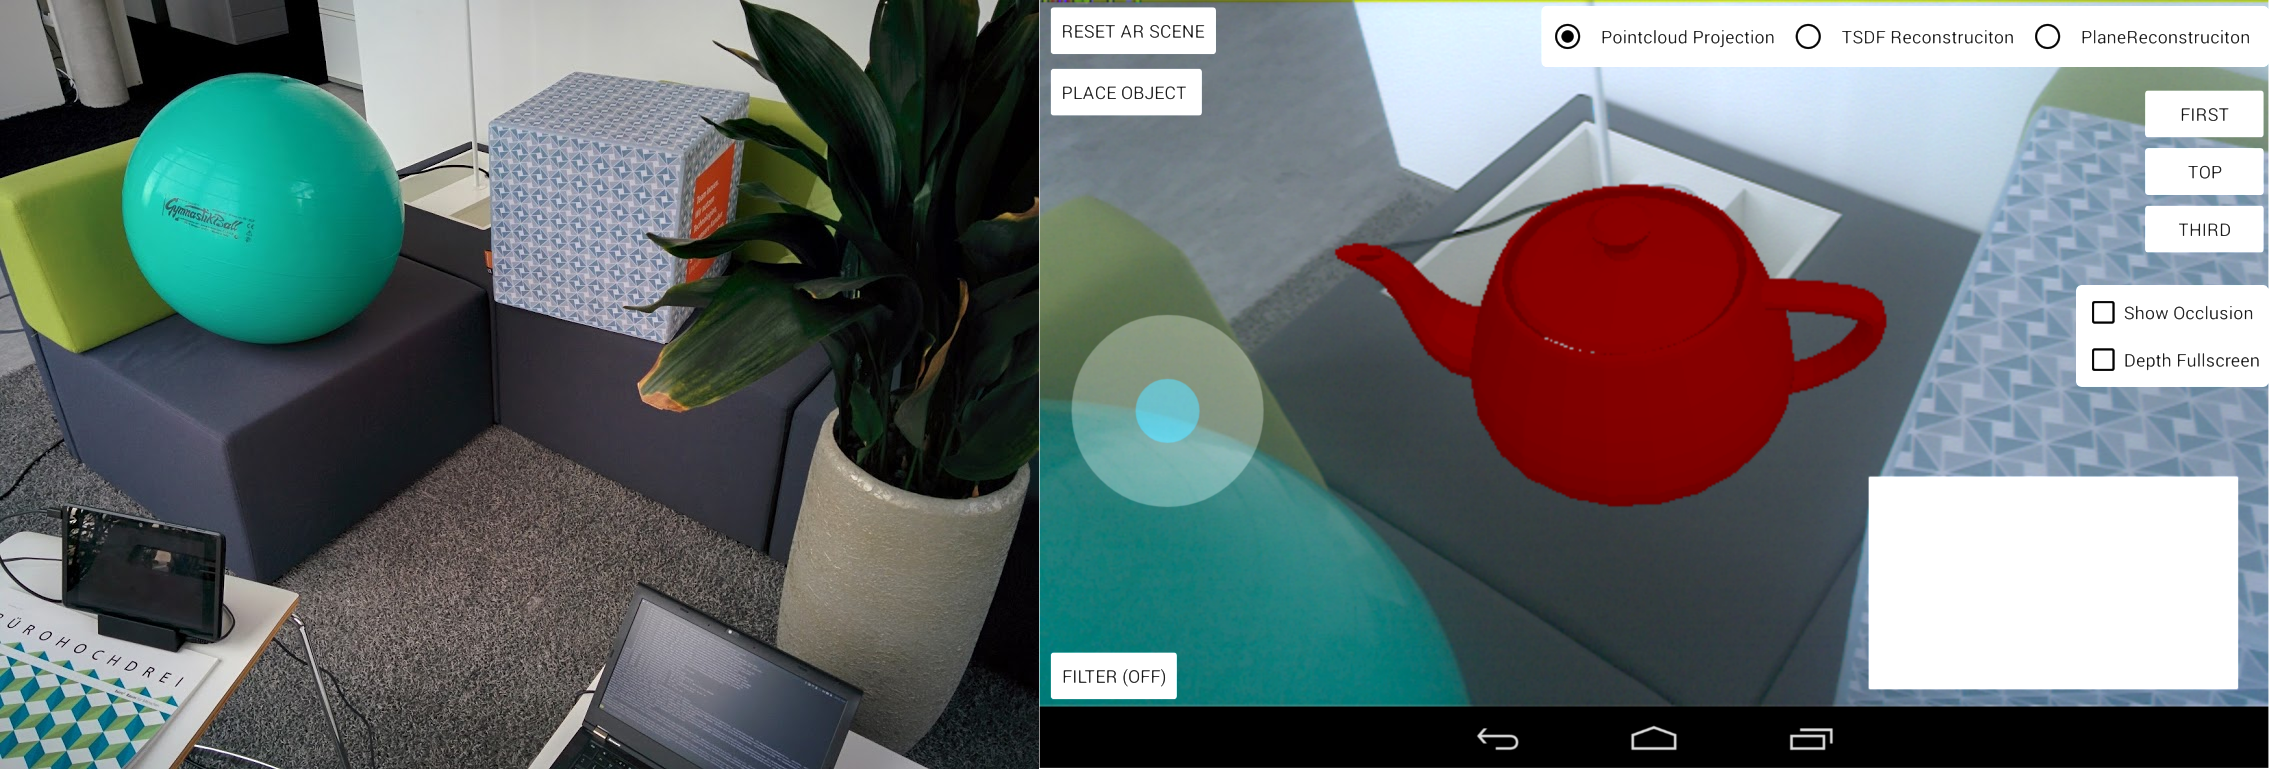
\includegraphics[width=1.0\textwidth]{content/images/evaluation/static-scene.png} 
  \caption{Links: Erste statische Szene mit einem Hocker und einem Sitzball. Rechts: Platzierung des virtuellen Objekts. }
  \label{fig:static-scene}
\end{figure}

Die zweite gewählte Szene, welche in Abbildung \ref{fig:plant-scene} links zu sehen ist, soll als Herausforderung die Überdeckung von komplexeren Strukturen testen. Sie besteht daher aus einer Pflanze, die sich, wie rechts im Bild zu sehen, vor dem virtuellen Objekt befindet. Auch hier befindet sich das Project Tango Gerät in einem Stativ.

\begin{figure}[h]
  \centering
	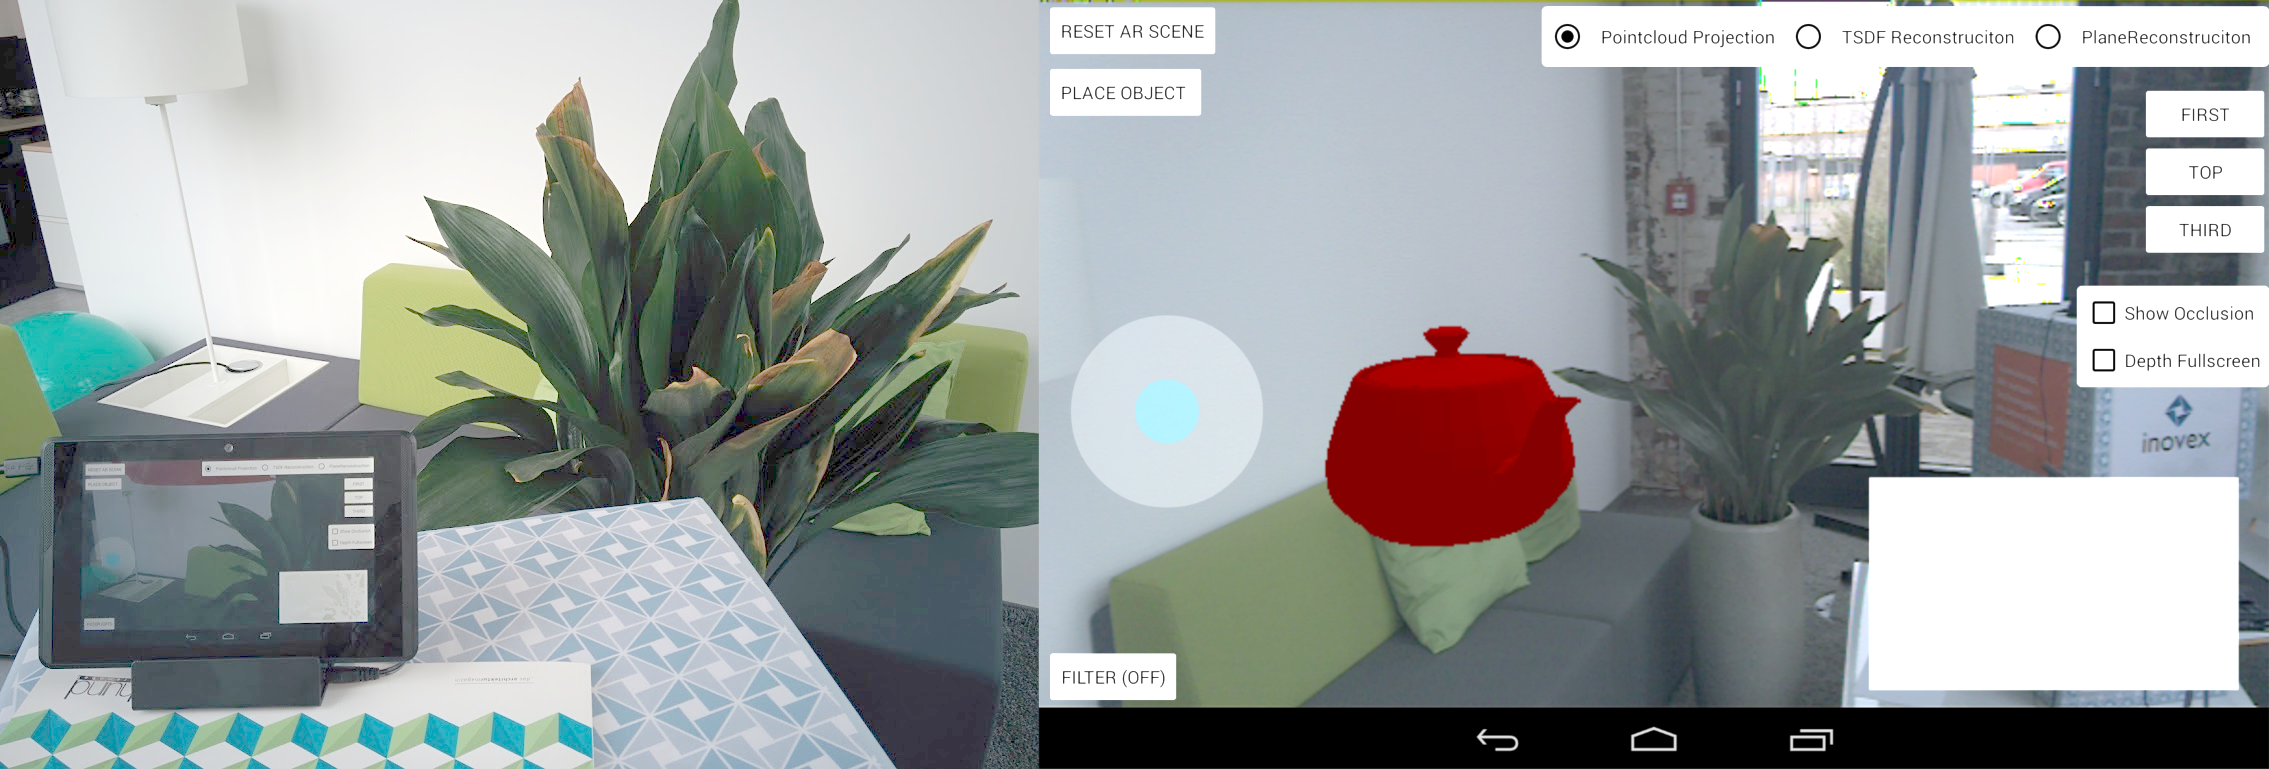
\includegraphics[width=1.0\textwidth]{content/images/evaluation/plant-scene.png} 
  \caption{Links: Zweite statische Szene mit einer Pflanze im Vordergrund. Rechts: Platzierung des virtuellen Objekts hinter der Pflanze. }
  \label{fig:plant-scene}
\end{figure}

Für beide Szenen sollen alle Kombinationen der Verfahren getestet werden. Somit ergeben sich sechs verschiedene Kombinationen, in denen die Pointcloud Projektion, die TSDF Rekonstruktion und die Ebenen Rekonstruktion jeweils mit und ohne dem Guided Filter getestet werden. Für alle Kombinationen soll ein gerendertes Bild und ein Tiefenbild mit dem virtuellen Objekt festgehalten werden. Zur Auswertung werden die jeweils gerenderten Ergebnisbilder \(p\) mit einem manuell zugeschnittenem Ergebnisbild  \(q\) für jeden Pixel \(i\) verglichen. Hierfür wird die Summe der absoluten Bilddifferenz wie in Gleichung \ref{eq:diff} bestimmt.

\begin{equation} \label{eq:diff}
d = \sum_i |p_i-q_i|
\end{equation}

\section{Durchführung der Tests}



\begin{figure}[h]
  \centering
	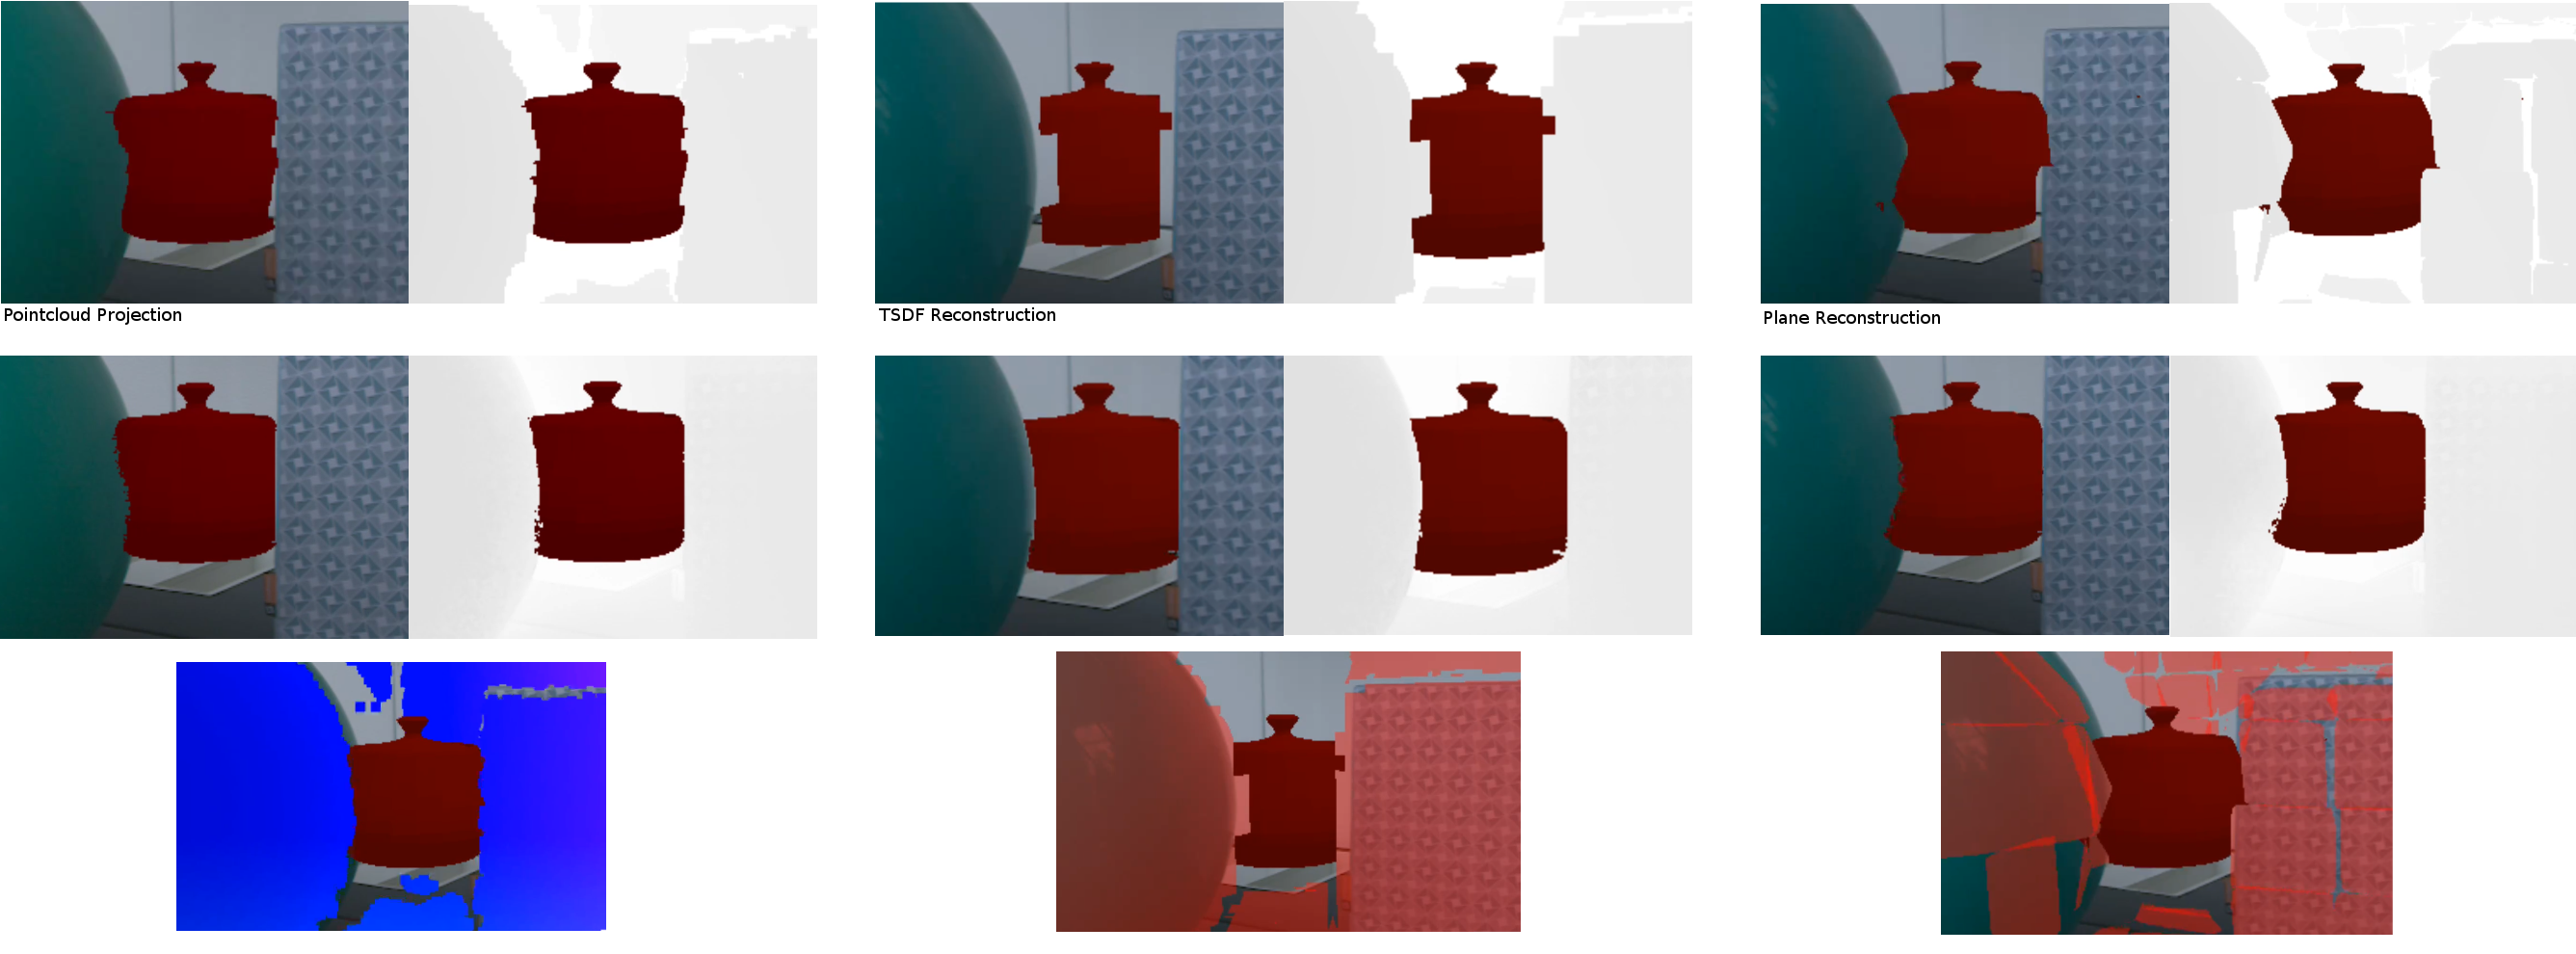
\includegraphics[width=1.0\textwidth]{content/images/evaluation/static_occlusion.png} 
  \caption{}
  \label{fig:static_occlusion}
\end{figure}

\begin{figure}[h]
  \centering
	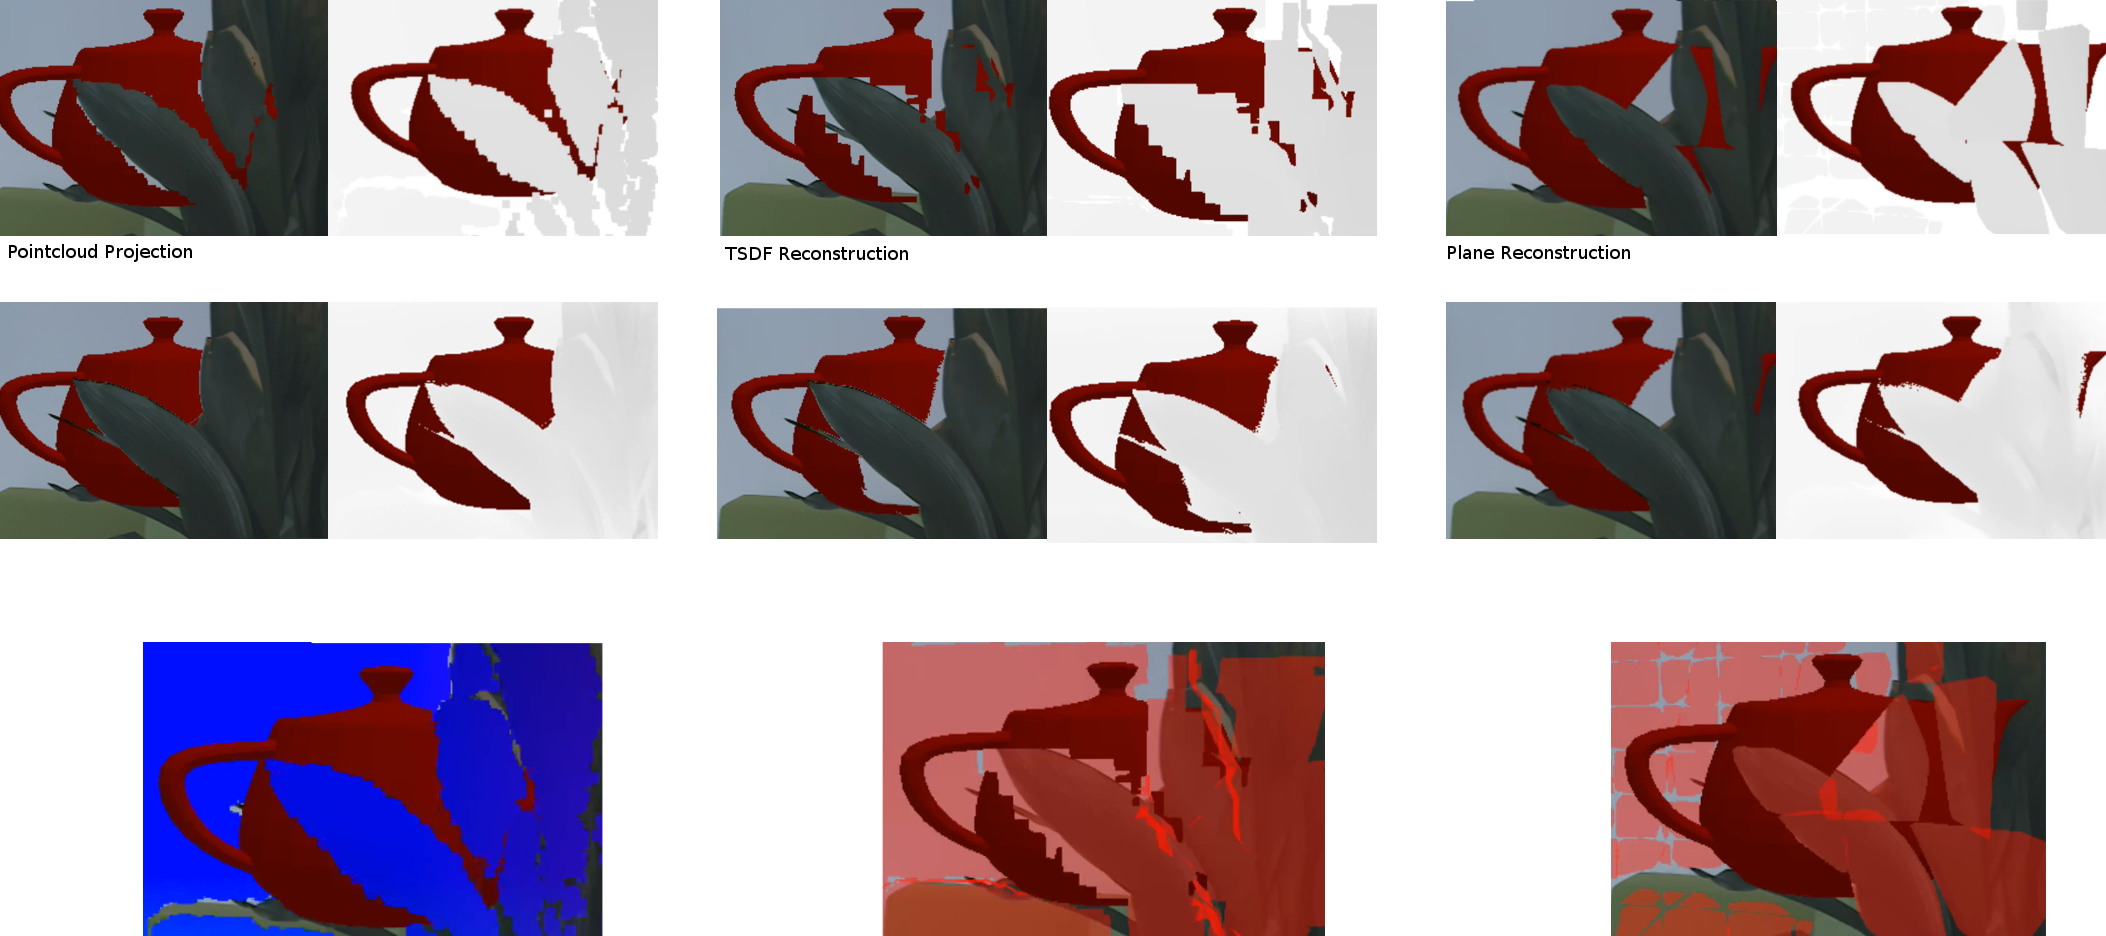
\includegraphics[width=1.0\textwidth]{content/images/evaluation/plant_occlusion.png} 
  \caption{}
  \label{fig:plant_occlusion}
\end{figure}

\section{Vergleich der Ergebnisse}

\begin{figure}[h]
  \centering
	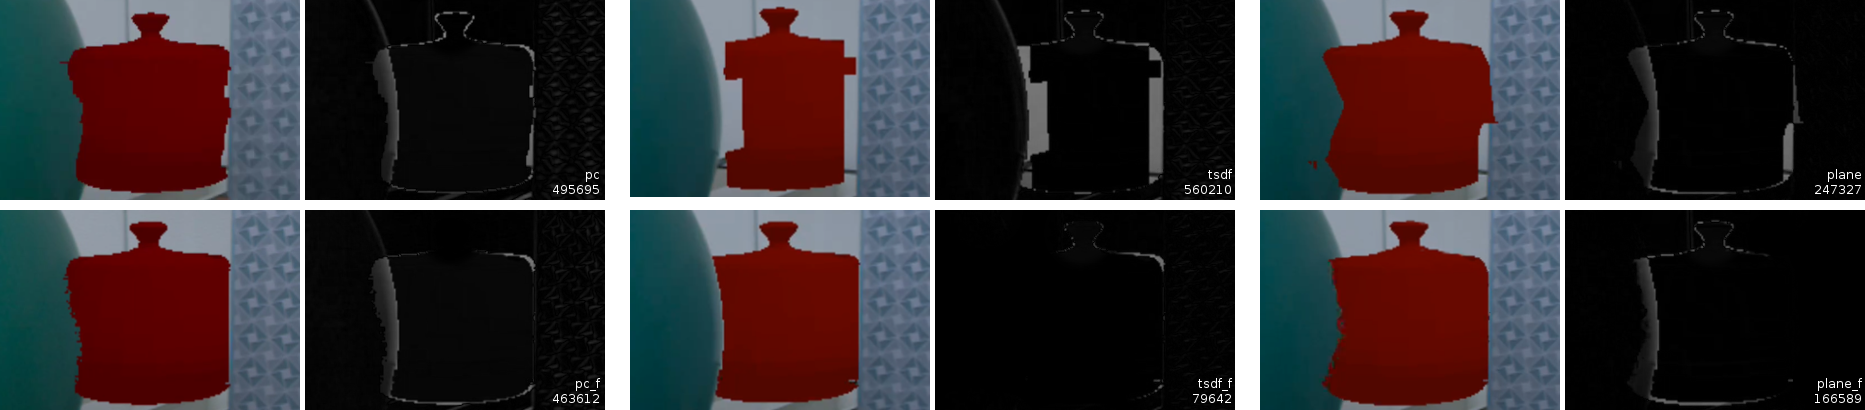
\includegraphics[width=1.0\textwidth]{content/images/evaluation/static_occlusion_results.png} 
  \caption{}
  \label{fig:static_occlusion_results}
\end{figure}

\begin{figure}[h]
  \centering
	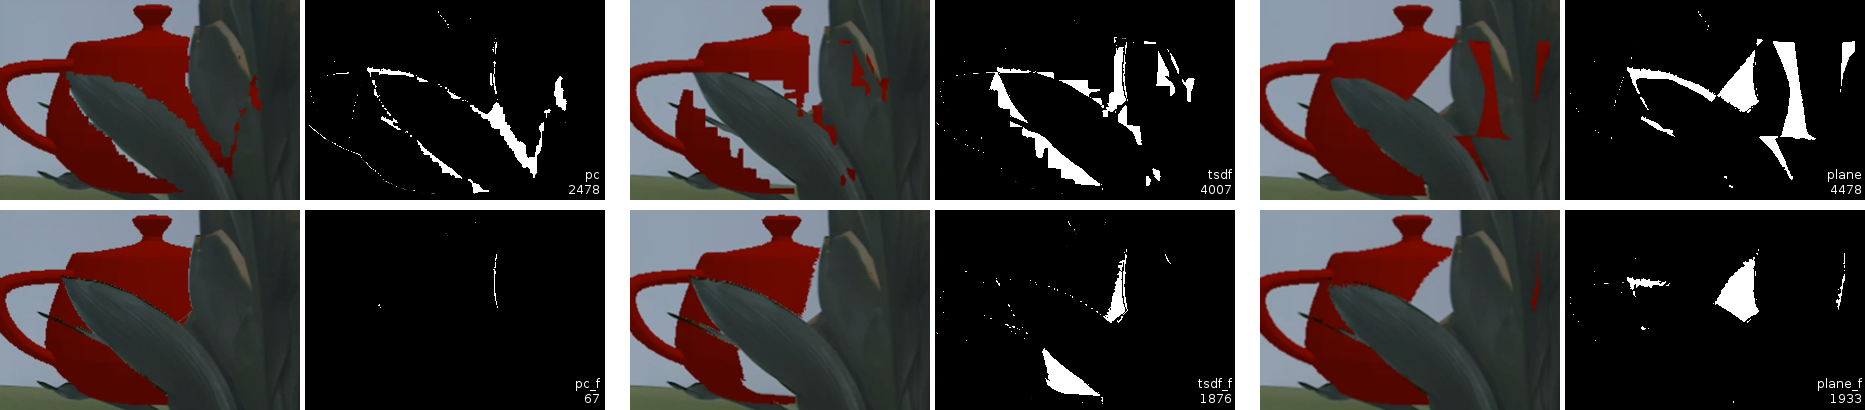
\includegraphics[width=1.0\textwidth]{content/images/evaluation/plant_occlusion_results.png} 
  \caption{}
  \label{fig:plant_occlusion_results}
\end{figure}



\begin{table}[]
\centering
\begin{tabular}{@{}rrrr@{}}
\toprule
                      & \textbf{\begin{tabular}[c]{@{}r@{}}Pointcloud \\ Projektion\end{tabular}} & \textbf{\begin{tabular}[c]{@{}r@{}}TSDF \\ Rekonstruktion\end{tabular}} & \textbf{\begin{tabular}[c]{@{}r@{}}Ebenen \\ Rekonstruktion\end{tabular}} \\ \midrule
\textbf{Szene 1}      & 499793                                                                    & 537532                                                                  & 300019                                                                    \\
\textbf{Szene 1 + GF} & 441672                                                                    & Referenz                                                                & 250254                                                                    \\
\textbf{Szene 2}      & 190317                                                                    & 460392                                                                  & 296190                                                                    \\
\textbf{Szene 2 + GF} & Referenz                                                                  & 334400                                                                  & 278334                                                                    \\ \bottomrule
\end{tabular}
\caption{Distanzwert zwischen dem Referenzbild und den Ergebnisbildern der Verfahren in der jeweiligen Szene}
\label{my-label}
\end{table}